\chapter{Graph Kernels}

\section{Bayes Factor}
A bayesian approach to model selection is to compare $p(M_1 | D)$ and $p(M_2 | D)$. $M_1, M_2$ are possible models of the data, e.g. $M_1 = \cG_{1D\; \GIRG}$ and $M_2 = \cG_{CL}$. $D$ is a single graph instance $G$, or alternatively a whole dataset of our 100 facebook graphs, assuming that they all come from the same generative model family. We have some prior of $p(M_1)$ vs $p(M_2)$, e.g. $50 : 50$, or for the possible different dimensional GIRGS some kind of decaying $p(1D\; \GIRG) > p(2D\; \GIRG) > p(3D\; \GIRG) > \dots$.
Putting this together,
\begin{equation}
  p(M_1 | D) = \frac{p(D | M_1) p(M_1)}{p(D)} 
  \;
  \implies
  \;
  \frac{p(M_1 | D)}{p(M_2 | D)} = \frac{p(D | M_1) p(M_1)}{p(D | M_2) p(M_2)}
\end{equation}
Hence model selection is done with the ratio $\frac{p(M_1 | D)}{p(M_2 | D)}$; this is called the Bayes Factor.
We will ignore the priors $p(M_1), p(M_2)$ for now, and focus on the likelihoods $p(D | M_1), p(D | M_2)$.



\paragraph{More rigorous bayesian model comparison}
In our case if $M_1$ is a 1D GIRG, and we've decided to fix e.g. $\alpha, e, \{w_u\}_{u \in V}$, and just vary $\theta = c, \{x_u\}_{u \in V}$, then we could Monte Carlo sample $\theta \sim p(\theta)$ from the prior to get an estimate, 
\begin{equation} \label{eq:incorrect_girg_model_likelihood}
  p(D| M_1) = p(G | \cG_{\text{d-}\GIRG}) = \int_\theta p(G | \theta, \cG_{\text{d-}\GIRG}) p(\theta | \cG_{\text{d-}\GIRG}) d\theta
\end{equation}
% $p(D | M_1) = p(G) = \int_\theta p(G | \theta) p(\theta) d\theta$, 
The simplified notation is dropping the $| M_1$ as we've fix into some dimensional GIRG universe, $\int_\theta p(G | \theta) p(\theta) d\theta$.

There's a problem here. Our data is a graph $D=G$. In the computation we actually need to inspect $p(G | \theta) = \sum_{\sigma} p(G' \stackrel{\sigma}{\cong} G | \theta) p(\sigma)$. Here $\sigma$ is a permutation of the node IDs. This is a confusing concept for sure. This is an abuse of notation - normally $p(G | \theta)$ is not a sum over permutations, but rather the probability of generating this exact graph. This will have to be contextually apparent.

Hence our simple MonteCarlo computation of $p(G | \theta, \GIRG) < p(G | CL)$ which was sad, is actually not quite valid. So Yay! We can still hope that the GIRG model is better than ChungLu, or at least bayesianly more likely.

To be concrete, let's say $G=(1,2), (2, 3), (2, 4), (2, 5)$. Then we say $G$ is isomorphic to $G'$ with permutation $\sigma= (1,4)$ ($G \stackrel{\sigma}{\to} G'$) where $G' = (4, 2), (2, 3), (2, 1), (2, 5)$. So the compuation is actually sample $\theta$,  then for each $\sigma \in S_n$ create $G'$ where $G$ is isomorphic to $G'$ with permutation $sigma$ ($G \stackrel{\sigma}{\to} G'$), and calculate $p(G' | \theta)$. Add these up and take the average.
Finally repeat for more different $\theta$ samples and take an outer average.


% \begin{tikzpicture}
%     \node[circle, draw] (1) at (0, 0) {1};
%     \node[circle, draw] (2) at (2, 0) {2};
%     \node[circle, draw] (3) at (1, 1.732) {3};
  
%     \draw[-] (1) -- (2);
  
% \end{tikzpicture}

\begin{figure}
    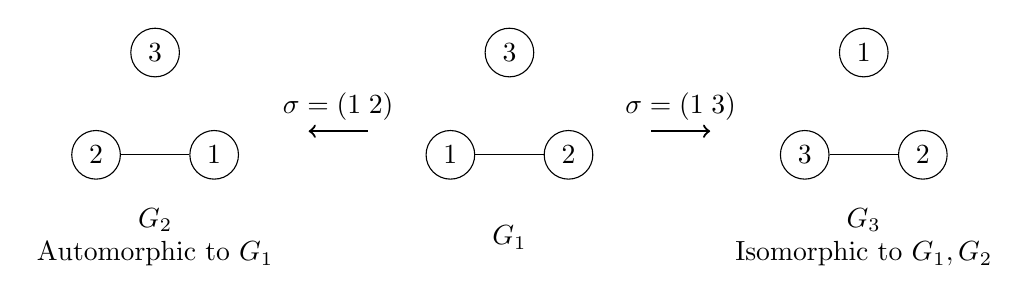
\begin{tikzpicture}[scale=1.5]
        % Graph 1
        \node[circle, draw] (g1v1) at (0, 0) {2};
        \node[circle, draw] (g1v2) at (1, 0) {1};
        \node[circle, draw] (g1v3) at (0.5, 0.866) {3};
    
        \draw[-] (g1v1) -- (g1v2);
    
        % Graph 2 (Automorphism)
        \node[circle, draw] (g2v2) at (3, 0) {1};
        \node[circle, draw] (g2v1) at (4, 0) {2};
        \node[circle, draw] (g2v3) at (3.5, 0.866) {3};
    
        \draw[-] (g2v2) -- (g2v1);
    
        % Graph 3
        \node[circle, draw] (g3v3) at (6, 0) {3};
        \node[circle, draw] (g3v2) at (7, 0) {2};
        \node[circle, draw] (g3v1) at (6.5, 0.866) {1};
    
        \draw[-] (g3v2) -- (g3v3);

        % % Arrows
        % \draw[->, thick] (g2v2) to[out=135,in=45] node[midway, above] {2 $\rightarrow$ 1} (g1v2);
        % \draw[->, thick] (g2v2) to[out=-135,in=-45] node[midway, below] {2 $\rightarrow$ 3} (g3v2);
      
        % Arrows
        \draw[<-, thick] (1.8, 0.2) -- node[midway, above] {$\sigma = (1\; 2)$} (2.3, 0.2);
        \draw[->, thick] (4.7, 0.2) -- node[midway, above] {$\sigma = (1\; 3)$} (5.2, 0.2);

    
        % Labels
        \node[align=center] at (0.5, -0.7) {$G_2$ \\Automorphic to $G_1$};
        \node[align=center] at (3.5, -0.7) {$G_1$};
        \node[align=center] at (6.5, -0.7) {$G_3$\\ Isomorphic to $G_1, G_2$};
    
    \end{tikzpicture}
    \caption{Example automorphic/isomorphic graphs}
\end{figure}
To be concrete, take an example graph $G = (V, E) = (\{1, 2, 3\}, \{(1,2)\})$. It's a "labelled graph". $G$ is isomorphic to any other labelled graph $H$ if they look the same if you anonymise the nodes. More formally, if $f: V(G) \to V(H)$ is a bijection mapping nodes to nodes, such that $u \sim v$ in $G$, $\iff f(u) \sim f(v)$ in $H$. So $G$ is isomorphic to $H$ with edge set $\{(1, 3)\}$. You can even say that it is automorphic to the graph $H$ with edge set $\{(2, 1)\}$, i.e. just switching nodes $1,2$.

So the setup is that with $G$ with 3 nodes, there are $3! = 6$ node ID permutations, each of which produces an isomorphic graph $G'$. For our particular $G$, we could group together these 6 isomorphic graphs $G'$ into 3 pairs of automorphic graphs.

Consider a simplified Chung-Lu / GIRG model where all nodes have the same weight $1$, and $\theta = (\vec{x}_1, \vec{x}_2, \vec{x}_3)$ of the three nodes. The Chung-Lu has identical $p(G')$ for each of the 6 ismorphisms. The GIRG  model does not - if $\vec{x}_1, \vec{x}_2$ are close, and $\vec{x}_3$ is far from both, then it awards higher probability to $G' = (V, \{(1,2)\})$ and $G' = (V, \{(2, 1)\})$. Furthermore both models always award the same probability to any equivalent class of automorphic graphs - this is because the adjacency matrix is the same for automorphic graphs, which is all that the models care about.

Unfortunately computing the $n!$ sized $\sum_{\sigma} p(G' \stackrel{\sigma}{\cong} G | \theta) p(\sigma)$ is infeasible for all but tiny graphs. 

There are some alternatives. One is to use a graph similarity kernel which compares two graphs $G, H$, giving some measure of how isomorphically similar they are. Apparently one more computable example is the random walk kernel. Therefore the idea would be to replace the incorrect $p(G | \cG_{\text{d-}\GIRG}) = \int_\theta p(G | \theta) p(\theta) d\theta$ with 
% $\mu(G) = \int_\theta k(G, G' \sim \cG_\theta) p(\theta) d\theta$. This is an idea.
$\mu(G) = E_{G' \sim \cG_{\text{d-}\GIRG}} \left [ k(G, G') \right ]$.

% Therefore the idea would be to replace the incorrect $p(G | \cG_{\text{d-}\GIRG}) = \int_\theta p(G | \theta, \cG_{\text{d-}\GIRG}) p(\theta | \cG_{\text{d-}\GIRG}) d\theta$ with $\mu(G) = E_{G' \sim \cG_{\text{d-}\GIRG}} \left [ k(G, G') \right ]$. This is an idea.

So when we say $p(G | \theta)$, we actually mean the probability of getting a graph $G'$ which is isomorphic to $G$, given parameters $\theta$.




\begin{figure}
    \centering

    \begin{subfigure}{0.49\textwidth}
      \centering
      \includegraphics[width=\linewidth]{figures/socfb-Amherst41-1d.png}
      \caption{$d=1$}
    \end{subfigure}
    \hfill
    \begin{subfigure}{0.49\textwidth}
      \centering
      \includegraphics[width=\linewidth]{figures/socfb-Amherst41-2d.png}
      \caption{$d=2$}
    \end{subfigure}
  
    \vspace{1em}
  
    \begin{subfigure}{0.49\textwidth}
      \centering
      \includegraphics[width=\linewidth]{figures/socfb-Amherst41-3d.png}
      \caption{$d=3$}
    \end{subfigure}
    \hfill
  
    \caption{MCMC runs for socfb-Amherst41, without failure rate}
    \label{fig:amherst_non_failure_mcmc}
\end{figure}

We see in \cref{fig:amherst_non_failure_mcmc} that Bayes Factor model comparison wise, 1D GIRGs are superior, even though according to edge accuracy, 2D GIRGs achieve a slight edge.


\section{Graph Kernel Introduction}
Graph Kernels provide a means for a similarity metric between graphs. They're ideally a positive semidefinite function $k: \Gamma \times \Gamma \rightarrow \mathbb{R}$, where $\Gamma$ is the set of all graphs. Such a function exists if and only if there is a corresponding feature map resentation of $\phi: \Gamma \to \cH_\phi$ where $\cH_\phi$ is a Hilbert space, and $k(G, G') = \langle \phi(G), \phi(G') \rangle_{\cH_\phi}$ is just an inner product.

Graph kernels give a simplified version of Blasius' classification framework. Blasius compares multiple different graph feature combination on which to train an SVM for distinguishing two graph datasets. Instead we can replace this with a single kernel which hopefully encapsulates sufficient relevant information on the graph. The question of which graph features to use then shifts to which graph kernel to use!

Another benefit of graph kernels is, as a similarity metric, they give easier direct comparison between graphs. As in the proposed paradigm in the previous section, we can directly compare the similarity of a real graph $G$ with two synthetic graphs $G_1, G_2$, produced from different models $M_1, M_2$. This is simply done by comparing $k(G, G_1)$ and $k(G, G_2)$ - the higher of the two is the more similar.


Graph Kernels have many uses, but we can use them in particular to help with bayesian model comparison, solving our issue of graph permutations.

A survey on graph kernels https://appliednetsci.springeropen.com/articles/10.1007/s41109-019-0195-3



We saw the equation $\mu(G) = E_{G' \sim \cG_{\text{d-}\GIRG}} \left [ k(G, G') \right ]$ in the previous chapter. We can Monte Carlo sample this expectation to get an estimate.

\subsection{Random Walk Kernel; Weisfeiler-Lehman Kernel}
There are many graph kernels to choose from. However given the relatively large size of our graphs, we opted to mainly test the Weisfeiler-Lehman Kernel. It has the benefit of running in $O(h|E|)$ time, where $|E|$ is the number of edges in the graph and $h$ is the number of iterations of the algorithm.

\subsection{Experiments}
we do the comparison

Cube Similarity Plots:
We fit alpha, c for a uniform cube GIRG for dimensions d=1-3, produce a graph, and look at similarity with real graph.
